\documentclass[conference,compsoc]{IEEEtran}

% *** CITATION PACKAGES ***
%
\ifCLASSOPTIONcompsoc
  % IEEE Computer Society needs nocompress option
  % requires cite.sty v4.0 or later (November 2003)
  \usepackage[nocompress]{cite}
\else
  % normal IEEE
  \usepackage{cite}
\fi
\usepackage[pdftex,
            pdfauthor={Yuejian Mo},
            pdftitle={SVM_11510511},
            pdfsubject={Report of project4}]{hyperref}

\usepackage{graphics}
\usepackage{graphicx}
\usepackage{amsmath}
\usepackage{algorithm, algorithmic}
\renewcommand{\algorithmicrequire}{\textbf{Input:}}
\renewcommand{\algorithmicensure}{\textbf{Output:}}
\usepackage{array}
\usepackage{url}
% correct bad hyphenation here
\hyphenation{op-tical net-works semi-conduc-tor}


\begin{document}
\title{Project 4: Support Vector Machine}

% author names and affiliations
% use a multiple column layout for up to three different
% affiliations
\author{\IEEEauthorblockN{Yuejian Mo  11510511}
\IEEEauthorblockA{Department of Biology\\
Southern University of Science and Technology\\
Email: 11510511@mail.sustc.edu.cn}}

% make the title area
\maketitle

\IEEEpeerreviewmaketitle

\section{Preliminaries}

Support vector machine, are supervised learning models with associated learning
algorithms that analyze data used for classification and regression analysis.
Given a set of training examples, each marked as belonging to one or the other
of two categories, an SVM training algorithm builds a model that assigns new
examples to one category or the other, making it a non-probabilistic binary
linear classifier.\cite{1} If the dataset are points in space, we can find out
an gap separate dataset into two part by using SVM.

\begin{figure}[ht!]
\centering
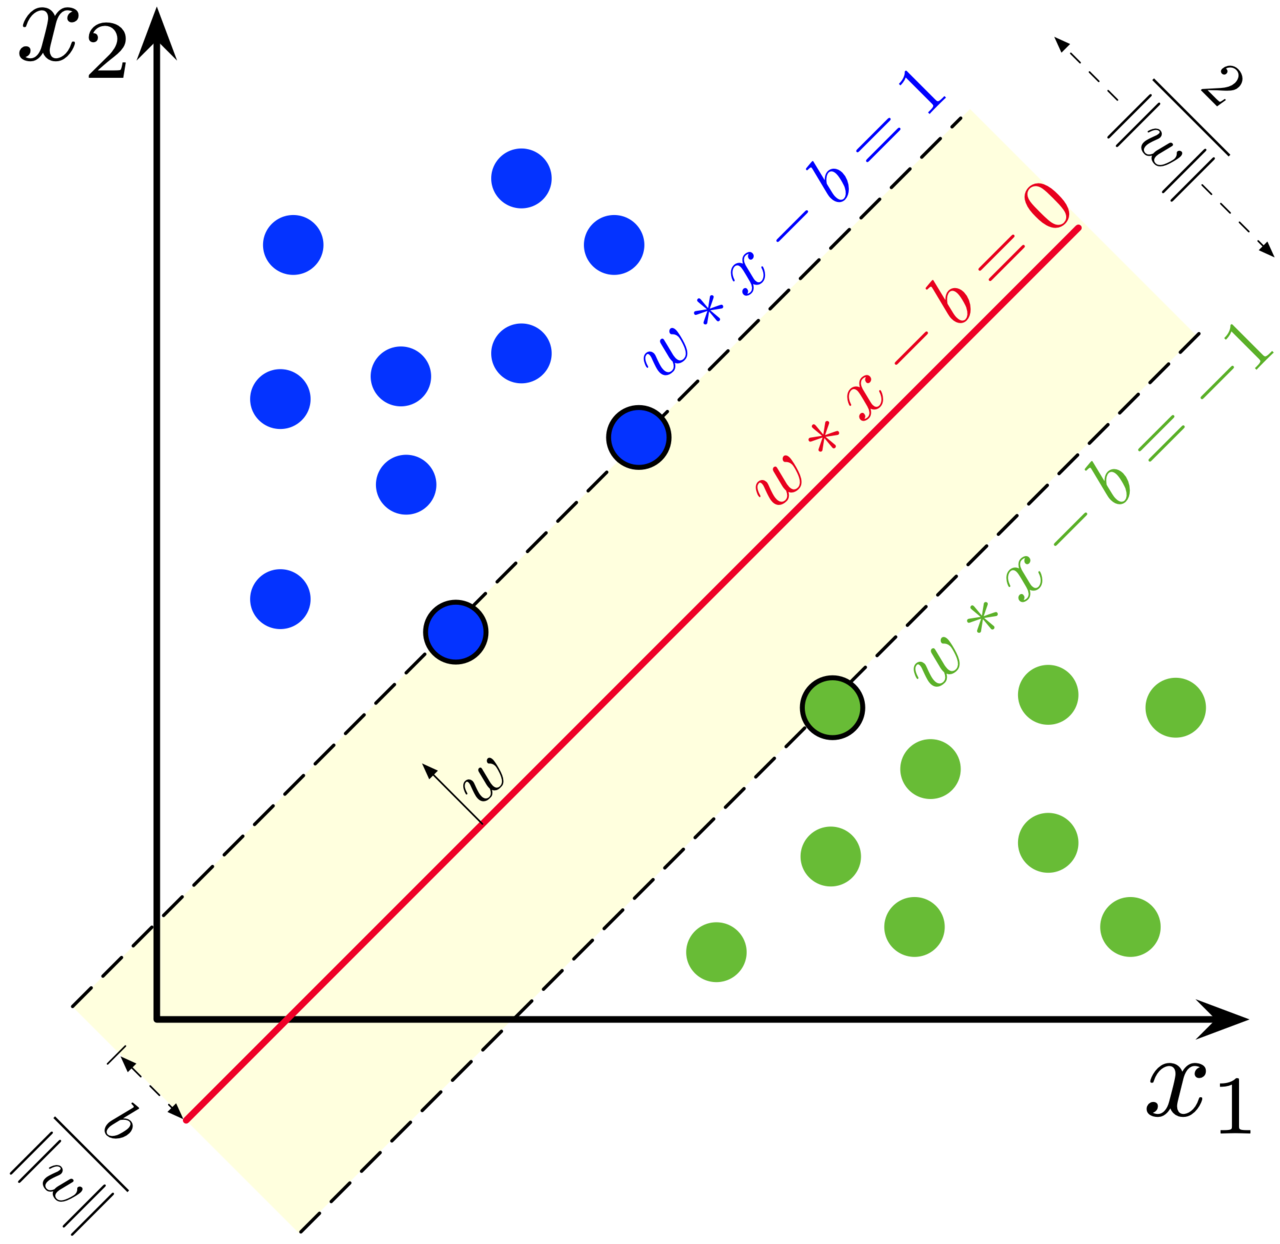
\includegraphics[width=0.65\linewidth]{1280px-SVM_margin.png}
\caption{Separate data points into two part using SVM(from Larhmam) 
	\label{SVM demostrains}}
\end{figure}

The original SVM algorithm was invented by Vladir N. Vapnik and
Alexey Ya. Chervonenkis in 1963. During the development, SVM are able to deal
with more tasks. SVM are used in text and hypertext categorization,
classification of images, hand-written characters recognition and proteins
classification.

In this project, I use SVM with random gradient descent to classify training
data almost correctly. 


\subsection{Software}
This project is written by Python 3.7 with editor Vim. Numpy, os, time,
random, sys and argparse library are used.

\subsection{Algorithm}
Model question with SVM. To optimal time cost and current of solution, random
gradient descent is used.

\section{Methodology}
Training set contain 1334 sample, and each sample contain 10 features and 1
label. With the help of other mathematical tools, training data show that
it can be classified in linear model. So, SVM model is used as training
model.

For most common and basic SVM(Figure 1), linear SVM uses two parallel vector
$w\cdot{x}-b=1$
and $w\cdot{x}-b=-1$ to separate dataset $x$ into two parts, where $x$ is
$m*n$ matrix with $n$ training samples of $m$ features, $w$ is a $m$ dimension
vector of SVM parameters and $b$ also is parameter of SVM. The rule is that gap
between two support vector don't exist any points expect of on the vectors.
To optimal correctness of classification, enlarging the distance
$\frac{2}{||w||}$ between two support vector is one of method. It belong to
convex optimization problem as following:

$${min}_{w,b}\frac{||w||^2}{2}$$
$$s.t. y_i((w\cdot{x_i})+b) \le1, i=1,...,n$$

To train data, we use loss function(also called cost function) to measure the
difference between SVM's prediction and actual labels. Each training, SVM try
to decrease the value of loss function. 

$$ L(w,b)=\sum^n_i=1 max(0, 1-y_i((w_i, x_i)+b)) $$

Then Gradient descend is used to update the feature weight matrix $w$. Each
training, gradient descend promote loss function decrease by moving to
opposite direction of gradient. In order to reduce the time cost to update
$w$ with whole dataset, we always to choose part of dataset in random.

$$ w = w -\alpha\frac{\partial L(w,b)}{\partial w}$$
$$ \frac{\partial L(w,b)}{\partial w} = -y_i x_i, if 1-y_i((<w,x>+b)>=0), otherwise 0$$

In above formula, $\alpha$ is the learning rate,
which determine the moved distance in each update. In this project, learning
rate always is updated during training, where learning rate being slower and
slower.

$$w = w -\beta \alpha \frac{\partial L(w,b)}{\partial w}$$

In practical, we add one more direction at the end of each sample$x_i$.
Final $w$ combine original $w$ and $b$ together. So $x$ is a $(m+1)n$ matrix,
and $w$ is a $m+1$ vector.

To avoid over fitting, k-fold cross validation is used. Whole training dataset
is divided into 10 parts in equal in random. Each time, one part from 10 parts
is chosen as test dataset, other 9 part as training dataset. Finally, the
average of all $w$ in 10 model is final $w$.

After training by SVM, $w$ and $b$ is final result, which can predict the label
of test dataset.

\subsection{Representation}
Some main data are maintain during process: \textbf{time\_budget},
\textbf{node\_num}, \textbf{graph\_cp}, \textbf{graph\_pc}, \textbf{incoming}.
Others data would be specified inside functions.

\begin{itemize}
	\item \textbf{x}: $(m+1)n$ dimensions numpy matrix to store input data.
  \item \textbf{y}: $n$ dimensions numpy matrix of label of input data.
  \item \textbf{w}: $m+1$ dimensions numpy matrix of weight and bias of SVM
	  parameters.
\end{itemize}


\subsection{Architecture}
Here list main functions of \textbf{SVM.py} in given code:
\begin{itemize}
    \item \textbf{init}: load train data to $x$, $y$; load time limit; initialize
	    parameter matrix $w$.
    \item \textbf{cal\_sgd}: Update $w$ using gradient descent.
    \item \textbf{train}: Train $w$ from train data data $x$, $y$.
    \item \textbf{predict}: Predict label of test data
    \item \textbf{\_\_main\_\_}: Main function
\end{itemize}

The \textbf{SVM.py} is executed locally.

\subsection{Detail of Algorithm}
Here describes some vital functions.
\begin{itemize}
    \item \textbf{init}: load train data and initial parameters
    \begin{algorithm}[H]
     \caption{int}
     \begin{algorithmic}[1]
     \renewcommand{\algorithmicrequire}{\textbf{Input:}}
     \renewcommand{\algorithmicensure}{\textbf{Output:}}
     \REQUIRE $input\_file\_name, time\_limit$
     \ENSURE $x, y, w$
     \STATE open $input\_file\_name$ as $file$
     \STATE create set $data$
     \FOR {each line in $file$}
          \STATE split line, then package and append to $data$
     \ENDFOR
     \STATE transform set $data$ to matrix $x$
     \STATE $y \leftarrow x[:,-1]$ 
     \STATE $x[:, -1] \leftarrow 1$
     \STATE initialize $w$ in uniform distribution with length of $m+1$. 
     \RETURN $x, y, w$
     \end{algorithmic}
   \end{algorithm}

   \item \textbf{cal\_sgd}:Update $w$ using gradient descent
     \begin{algorithm}[H]
     \caption{cal\_sgd}
     \begin{algorithmic}[2]
     \renewcommand{\algorithmicrequire}{\textbf{Input:}}
     \renewcommand{\algorithmicensure}{\textbf{Output:}}
     \REQUIRE $x_i, y_i, w, \alpha, \beta$
     \ENSURE $w_{updated}$ 
     \IF {$y_i(x_i\cdot{w}) < 1$}
	     \STATE $w_{updated} = w - \beta(\alpha w - y_ix_i)$
     \ELSE
	     \STATE $w_{updated} = w - \beta\alpha yi$
     \ENDIF
     \RETURN $w_{updated}$
     \end{algorithmic}
     \end{algorithm}

  \item \textbf{train}: Train $w$ with data $x, y$
    \begin{algorithm}[H]
     \caption{train}
     \begin{algorithmic}[3]
     \renewcommand{\algorithmicrequire}{\textbf{Input:}}
     \renewcommand{\algorithmicensure}{\textbf{Output:}}
     \REQUIRE $x, y, w,\beta, \alpha$
     \ENSURE  $w$
     \STATE $t \leftarrow 0$
     \WHILE{ running time don't exceed ordered time}
	     \STATE reorder $x$ and $x$ in the same time
	     \STATE $loss \leftarrow 0$ 
	     \STATE $t \leftarrow t+1$
	     \STATE $\beta = 1/(\alpha t)$
	     \FOR{ each sample $x_i$ and $y_i$ in training data}
		  \STATE $w = cal\_sgd(x_i, y_i, w, \beta, \alpha)$
	     \ENDFOR
     \ENDWHILE
     \RETURN $w$
     \end{algorithmic}
     \end{algorithm}
 
 \item \textbf{predict}: Predict the label of test data
     \begin{algorithm}[H]
     \caption{predict}
     \begin{algorithmic}[4]
     \renewcommand{\algorithmicrequire}{\textbf{Input:}}
     \renewcommand{\algorithmicensure}{\textbf{Output:}}
     \REQUIRE $test\_file, w$
     \ENSURE  $label\_set$
     \STATE open $test\_file$ as $file$
     \STATE create set $test\_data$
     \FOR {each line in $file$}
          \STATE split line, then package and append to $test\_data$
     \ENDFOR
     \STATE transform set $test\_data$ to matrix $test\_set$
     \STATE append 1 at each end of column
     \STATE $label\_set \leftarrow  sgn(test\_set\cdot{w})$
     \RETURN $label\_set$
     \end{algorithmic}
     \end{algorithm}
 
 \item \textbf{\_\_main\_\_}: main control flow
	 \begin{algorithm}[H]
	\caption{\_\_main\_\_}
	\begin{algorithmic}[5]
 	\renewcommand{\algorithmicrequire}{\textbf{Input:}}
        \renewcommand{\algorithmicensure}{\textbf{Output:}}
	\REQUIRE 
	\ENSURE
	\STATE pass through $time\_limit$, train dataset, test dataset
	\STATE $init$
	\STATE use 10-hold cross validation train $w$
	\STATE use $predict$ with test data set to predict final result
	\end{algorithmic}
        \end{algorithm}
 	
\end{itemize}


\section{Empirical Verification}
Empirical verification is verified offline with given dataset. K-fold
cross-validation is used to verify and choose best result. In most of
case, the correctness is above 90 percent.

\subsection{Design}

Random gradient descent return in reasonable time than simple gradient
descent algorithm.

K-fold cross validation maybe reduce chance of overfitting, but it reduce
the iteration of single gradient descent. Although, training without cross
validation performance better, cross validation result still is suitable
for unknown dataset.

Training time also determine the performance of final result, which seem
that more time is flavor. 


\subsection{Data and data structure}
For the convenience, matrix are used widely to store train set, test set and
features matrix.

\subsection{Performance}
Following table show different performance with different parameters. Offline
test perform at Fedora 29 with $Intel^{®}$ Xeon(R) CPU E5-1680 v3@3.20GHz and
32GiB memory.

Here are 10-fold cross validation.
\begin{center}
   \begin{tabular}{| l | l |l |}
   \hline
   Run Time(s)  &Iteration     &Correctness   \\ \hline
    10           &10*66        & 95.3523  \\
    20           &10*146       & 98.0510  \\
    30           &10*226       & 97.8260  \\
    60           &10*440       & 98.4258  \\
   \hline
   \end{tabular}
\end{center}

Here are training without 10-fold cross validation.
\begin{center}
   \begin{tabular}{| l | l |l |}
   \hline
   Run Time(s)  &Iteration     &Correctness   \\ \hline
    10           &670        & 97.2264  \\
    20           &1356       & 98.3759  \\
    30           &2064       & 97.9760  \\
    60           &4176       & 98.8006  \\
   \hline
   \end{tabular}
\end{center}


% Table of difference problem

\subsection{Result}
Best model classify data set at 99.6 percent of correctness.

\subsection{Analysis}
% Analysis different parameter's results
During training, most time cost is iteration of update $w$.

The cost of random gradient descent.


\section*{Acknowledgment}
Thanks TA Yao Zhao who explain question and provide general method to solve it.
And I also thanks for Kebing Sun discuss and share the idea about algorithm.

\bibliographystyle{IEEEtran}
\begin{thebibliography}{1}
\bibitem{1}
Wikipedia contributors, [Online], Available: https://en.wikipedia.org/wiki/Support\_vector\_machine, [Accessed: 31-Dec-2018].
\end{thebibliography}

% that's all folks
\end{document}


